    % \documentclass[handout,xcolor=pdftex,dvipsnames,table]{beamer}
    \documentclass{beamer}

    \usepackage{amsmath}
    \usepackage[english,brazil]{babel}
    \usepackage[utf8x]{inputenc}
    \usepackage{graphicx}
    \usepackage{url,color,ae}
    \usepackage{listings,color,upquote}
    \usepackage[T1]{fontenc}
    \usepackage[small]{caption}

    \hypersetup{pdftitle={IFSC - Campus Sao Jose},
	    pdfsubject={Telecomunicacoes}
    }



    %--------- Insercao de codigo fonte nos slides --------------------%
    \definecolor{hellgelb}{rgb}{1,1,0.9}
    \definecolor{colKeys}{rgb}{0,0,0}
    \definecolor{colIdentifier}{rgb}{0,0,0.9}
    \definecolor{colComments}{rgb}{.4,.4,.4}
    \definecolor{colString}{rgb}{0,0,0.6}

    % Comando: \java
    \newcommand{\java}
    {\lstset{language=java,basicstyle=\ttfamily\footnotesize,tabsize=3,frame=single,
    showtabs=false,showspaces=false,firstnumber=last,numbers=left,numberstyle=\tiny,
    linewidth=0.98\linewidth,xleftmargin=21pt,tab=$\to$,float=tbph,extendedchars,
    breaklines,showstringspaces=false,identifierstyle=\color{colIdentifier},
    keywordstyle=\color{colKeys},stringstyle=\color{colString},commentstyle=\color{
    colComments},backgroundcolor=\color{hellgelb},columns=flexible,captionpos=b,
    aboveskip=\bigskipamount}}

    % Comando: \shell
    \newcommand{\shell}
    {\lstset{language=csh,basicstyle=\ttfamily\footnotesize,tabsize=3,frame=single,
    showtabs=false,showspaces=false,firstnumber=last,numbers=left,numberstyle=\tiny,
    linewidth=0.98\linewidth,xleftmargin=21pt,tab=$\to$,float=tbph,extendedchars,
    breaklines,showstringspaces=false,identifierstyle=\color{colIdentifier},
    keywordstyle=\color{colKeys},stringstyle=\color{colString},commentstyle=\color{
    colComments},backgroundcolor=\color{hellgelb},columns=flexible,captionpos=b,
    aboveskip=\bigskipamount}}

    % ------------------ TEMA ---------------------------------------------%

    \usetheme[numbers,totalnumber,compress]{Madrid}
    % \usetheme{Warsaw}
    % \usetheme{Boadilla}
    % \usetheme{CambridgeUS}
    % \usetheme{Montpellier}
    % \usetheme{Hannover}
    % \usetheme{Dresden}


    \definecolor{azulescuro}{rgb}{0.3,0.42,0.601}  
    \definecolor{verde}{rgb}{0.55,0.78,0.25} 
    \definecolor{kugreen}{RGB}{50,93,61}
    \definecolor{kugreenlys}{RGB}{132,158,139}
    \definecolor{kugreenlyslys}{RGB}{173,190,177}
    \definecolor{kugreenlyslyslys}{RGB}{214,223,216}
    
    \usecolortheme[named=kugreen]{structure}
    \useinnertheme{circles}

    \setbeamertemplate{footline}[frame number]
    \beamertemplatenavigationsymbolsempty
    % ------------------------------------------------------------------ %

    \logo{
\includegraphics[width=.5cm]{figs/logo-ifsc.pdf}}






    % -------------------- Titulo -----------------------------------%

    \title{Projeto de instalação de uma emissora de radiodifusão sonora em frequência modulada, no município de São Pedro de Alcântara}
    \subtitle{}
    \author[Guilherme Bilbao Soares da Silva]{Guilherme Bilbao Soares da Silva\\Jaci Destri}
    \institute[IFSC]{
    Instituto Federal de Santa Catarina -- IFSC\\
    Campus São José \\
    \url{}
    }

    \date{Julho de 2013}


    % -------------- Início do documento ------------------ %
    \begin{document}

    \begin{frame}
	    \maketitle
    \end{frame}

    \frame{\frametitle{Conteúdo Programático}
    \tableofcontents}

    %\AtBeginSection[]{
    % \frame{
      %  \frametitle{Índice}
      % \tableofcontents[current,currentsection]
      %}
    %}

    \section{Motivação}
    \begin{frame}
    \frametitle{Motivação}
      \begin{itemize}
      \item Adquirir maiores conhecimentos em radiotransmissão;
      \item Estudo e compreensão das normas técnicas;
	\item A norma técnica sofre adaptações;
	\item Servir como referência para outros projetos/estudos.
	\end{itemize}

    \end{frame}


    \section{Proposta}

    \begin{frame}
	    \frametitle{Proposta}


	    Projeto de uma emissora FM num cenário real,
	    seguindo os procedimentos solicitados pela resolução
	    e normas vigentes para esta finalidade.
	    
	    Para isto, é utilizado o canal 218 (91,5 Mhz),disponível no plano básico,
	    no município de São Pedro de Alcântara.
	    
	  
    \end{frame}
    
    \begin{frame}
    
      \frametitle{Proposta}
      
      Objetivos Principais:
      
      \begin{itemize}
	  
	  \item Elaborar um documento que reúna todas a informações necessárias
	  para encontrar os resultados desejados neste estudo, e que também 
	  auxilie outros projetos similares futuramente.
	    
	  \item Apresentar os dados técnicos solicitados pela 
	    ANATEL, definidos através da Resolução n°67 e suas atualizações;
	    
	    
      \end{itemize}
    
    
    \end{frame}

    \section{Desenvolvimento}
      
    \begin{frame}
    
      \frametitle{Desenvolvimento}
      
          Informações e ferramentas necessárias para o desenvolvimento:
	\begin{itemize}
 
    
	  \item PBFM;
	  \item Resolução nº 67;
	  \item Recomendação UIT-R P.1546;
	  \item Ferramenta SIGAnatel.
      
      \end{itemize}
  
    \end{frame}
    
    \begin{frame}
    
      \frametitle{Desenvolvimento}
      
          Canal proposto:
	\begin{itemize}
	

	  \item Município de São Pedro de Alcântara;
	  \item Canal 218 (91,5 MHz) no PBFM;
	  \item Classe C;
	  \item Contorno protegido de 7,5 Km.
      
      \end{itemize}
  
    \end{frame}
    
        \begin{frame}
    
      \frametitle{Desenvolvimento}
      
      
	 Classificação da emissora:
      \begin{center}
      
           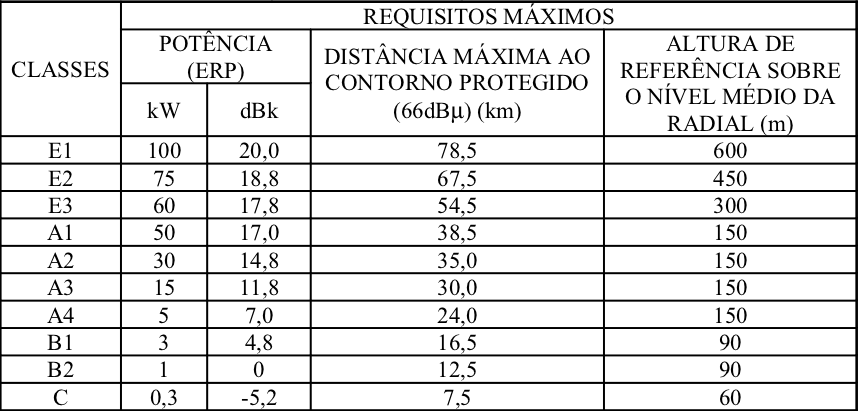
\includegraphics[width=.8\linewidth]{figs/tabelaClassificacaoEmissoras.png}		  		
        \end{center}
      
        
  
	\end{frame}
    
    \begin{frame}
    
      \frametitle{Desenvolvimento}
      
          Localização da base emissora:
	\begin{itemize}
	

	  \item 27º34'02.72''S, 48º48'33.71''O;
	  \item Área central do município;
	  \item 285 metros de altitude;
	  \item Ponto mais próximo ao local informado no PBFM.
      
      \end{itemize}
  
    \end{frame}
    
    \begin{frame}
    
      \frametitle{Desenvolvimento}
      NMR e NMT
      \begin{center}
      
           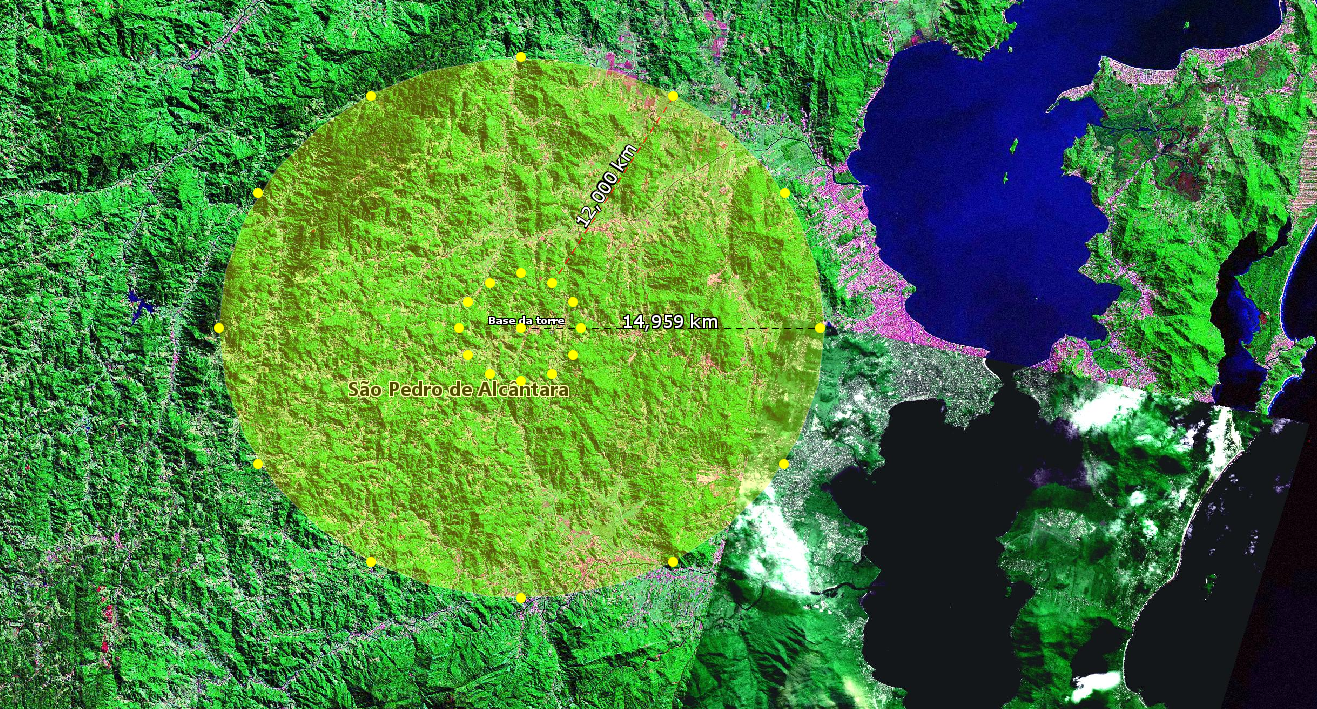
\includegraphics[width=.8\linewidth]{figs/radiais_detalhado.png}		  		
        \end{center}
  
      \end{frame}
    
     \begin{frame}
    
      \frametitle{Desenvolvimento}
      NMR e NMT
      \begin{center}
      
           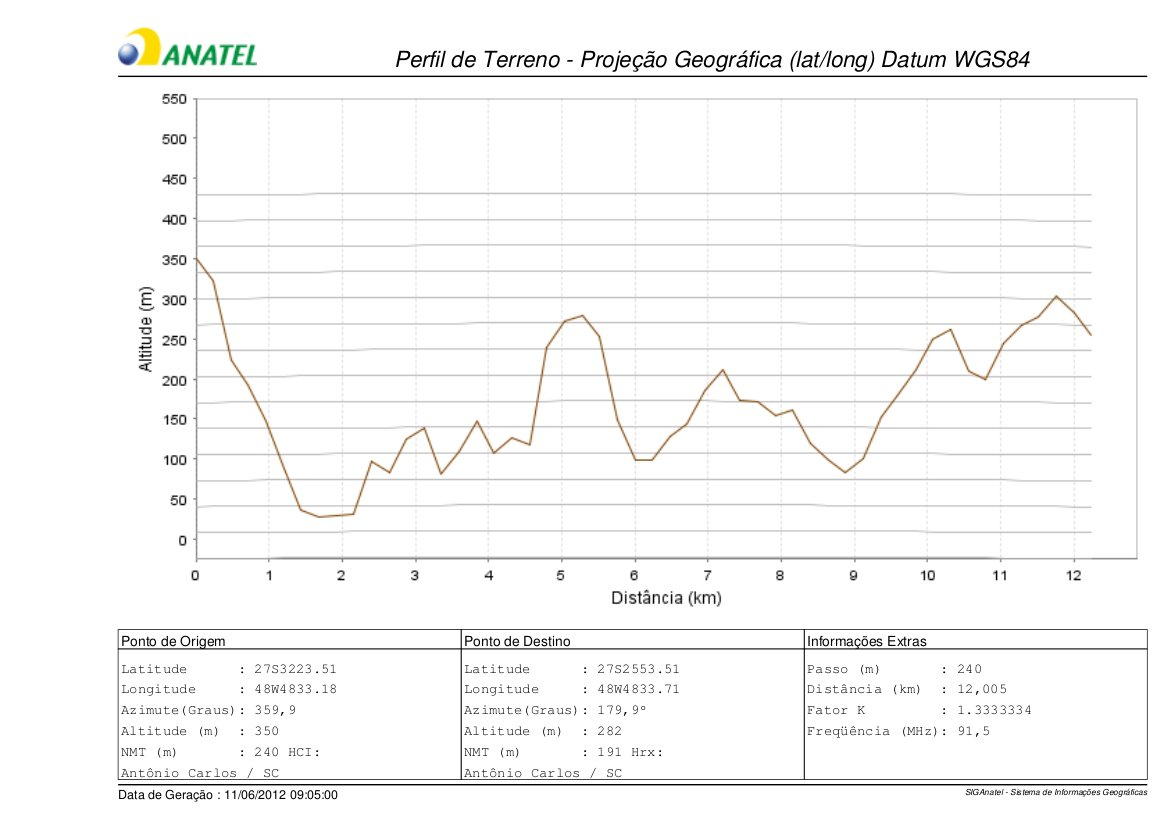
\includegraphics[width=.8\linewidth]{figs/nmt1_v2.jpg}		  		
        \end{center}
  
      \end{frame}
    
    
    
   % \begin{center}
    %\begin{array}{ll}
    %\includegraphics[width=.5\linewidth]{figuras/fou.png}		  		
    %\caption{}  & \includegraphics[width=.5\linewidth]{figuras/wa.png}		
    %  \caption{} 
    %\end{array}
    %\end{center}

    
    
    \section{Resultados}

    \section{Conclusões}
    \begin{frame}
    \frametitle{Conclusões}
    \begin{itemize}
    \item A Transformada Wavelet mostrou muito eficaz para a análise de sinais de
    voz;
    \item Após a utilização de outros métodos de obtenção do período de pitch, a
    Transformada Wavelet apresentou resultados similares aos valores do melhor
    método no domínio do tempo;
    \item Foi obtida uma taxa de acerto de 75\textdiscount para extração de pitch.
    \end{itemize}

    \end{frame}

    \section{Trabalhos Futuros}
    \begin{frame}
    \frametitle{Trabalhos Futuros}
      \begin{itemize}
	    \item Seria interessante o uso de outras técnicas para a implementação
    deste projeto como:
	    \begin{itemize}
		  \item Predição Linear (LPC);
		  \item O uso de filtros específicos;
		  \item Análise espectral do sinal;
		  \item Redes neurais Artificiais (RNA);
    \end{itemize}
    \end{itemize}
    \end{frame}

    \begin{frame}

      \frametitle{Obrigado pela atenção!}
      
      \begin{center}
      
    {\huge Dúvidas? } 

      \end{center} 
    
    \end{frame}

    \end{document}
